\section{Ergebnisse} % (fold)
    \label{sec:ergebnisse}
    \begin{table}[h]
        \centering
        \caption{t-Test-Ergebnisse}
        \label{tab:t_tests}
        \csvreader[tabular=rrr,
          table head=\toprule\centerIt{\textbf{Nullhypothese}} & \centerIt{\textbf{Sauer}} & \centerIt{\textbf{Salzig}}\\\midrule,
          /csv/separator=semicolon,
          head to column names,
          late after line=\\,
          late after last line=\\\bottomrule
          ]%
          {../Results/t_tests.csv}{H0=\H}%
        {\H & \pH & \NaCl}
    \end{table}

    \begin{figure}[h]
        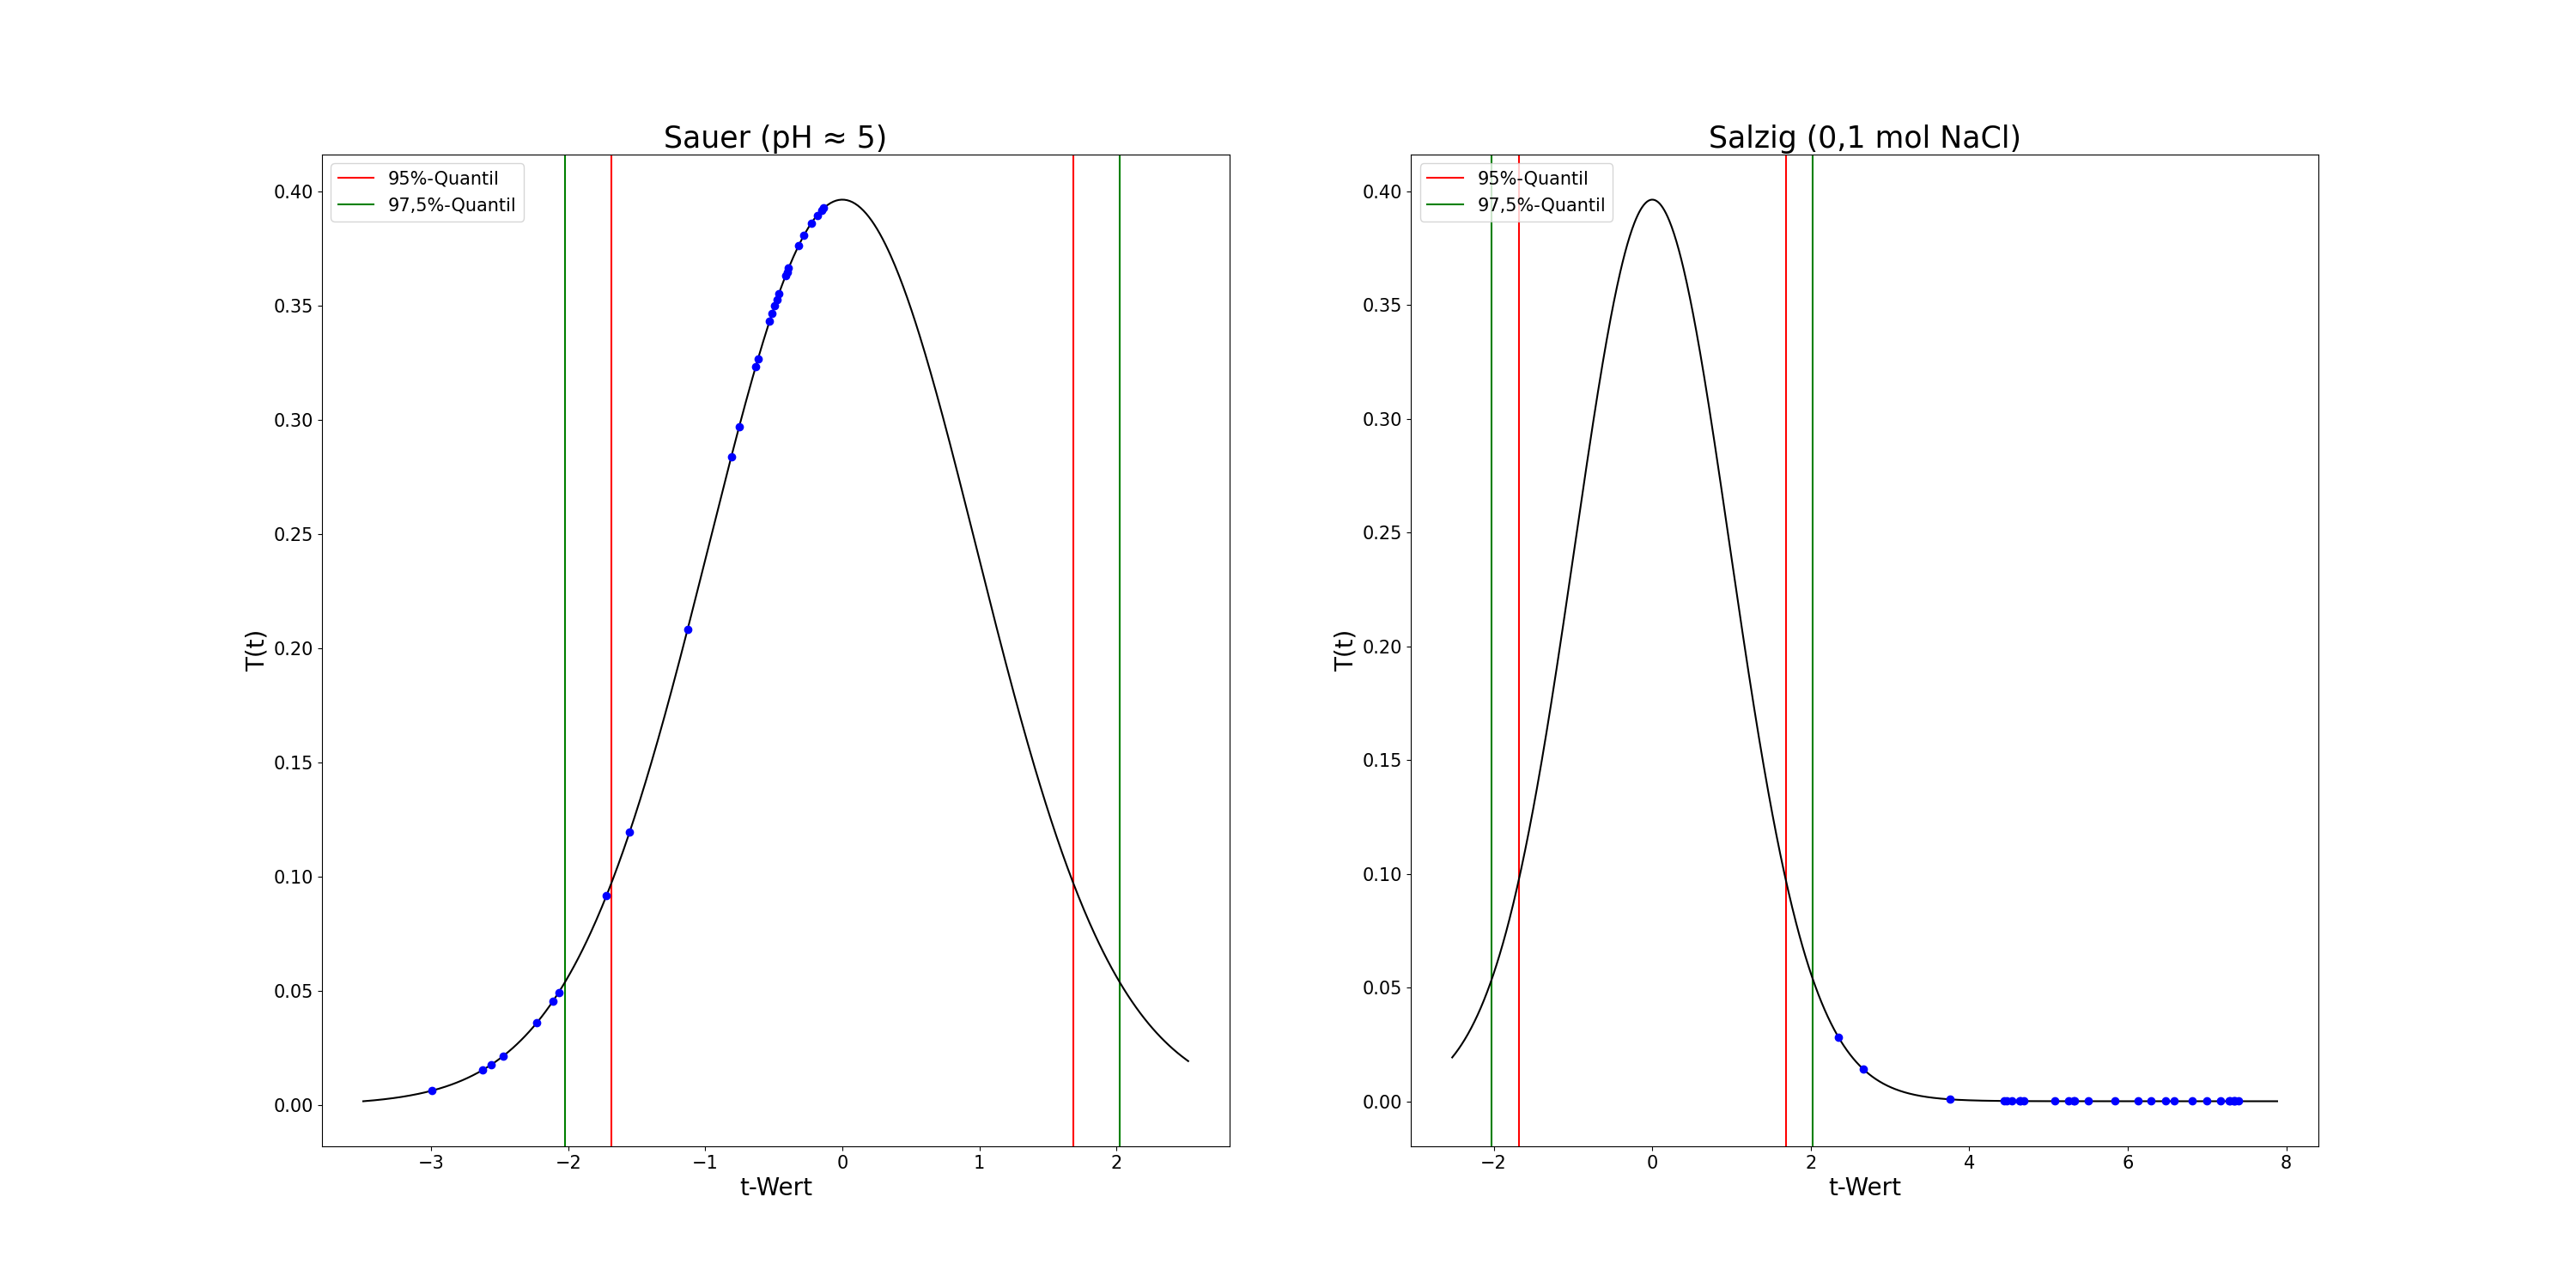
\includegraphics[width=1\textwidth]{t_tests.png}
        \caption{t-Tests}
        \label{fig:t_tests}
    \end{figure}
    In \autoref{tab:t_tests} und \autoref{fig:t_tests} sind die Ergebnisse der t-Tests gegenüber des neutralen Mediums dargestellt, tabellarisch und graphisch. Als Signifikanzniveau wurde hierfür ein \( \alpha \) von 5\% gewählt und dementsprechend für die Werte der t-Verteilung bei 38 Freiheitsgraden für einseitige Betrachtung 1,686 und die Zweiseitige 2,024\ \cite[vgl.][]{web:t-values}.
    \newpage

    \begin{figure}[h]
        \centering
        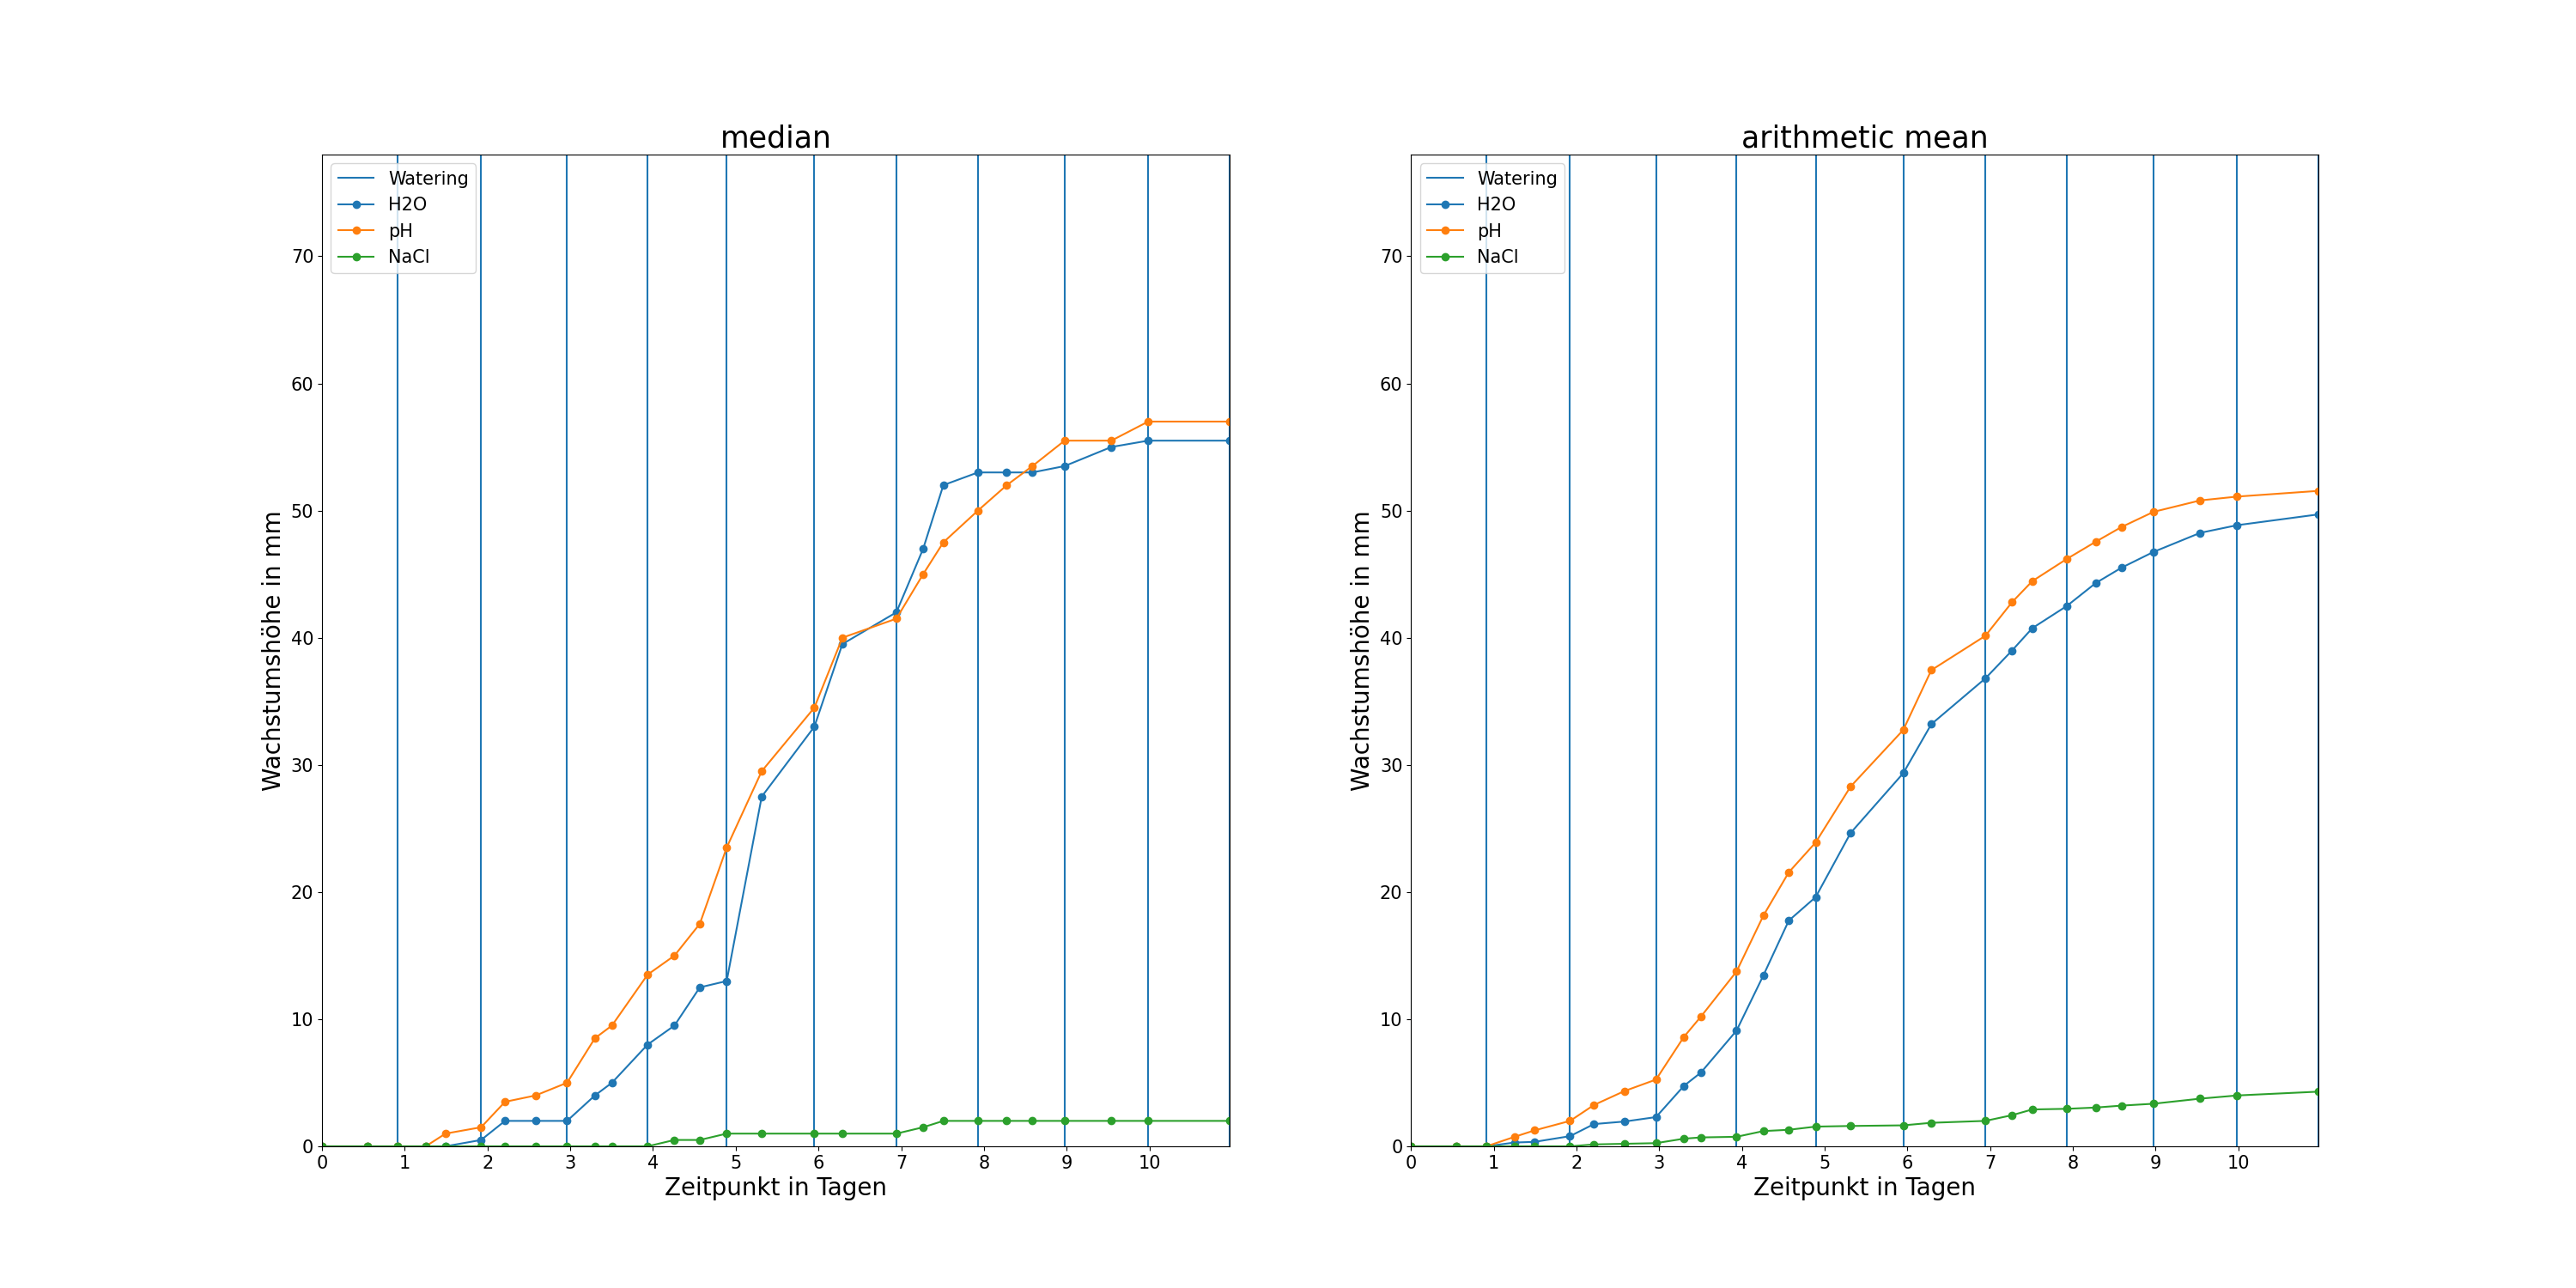
\includegraphics[width=.9\textwidth]{ScatterPlot.png}
        \caption{lineare Entwicklung der Messwerte}
        \label{fig:scat_plot}
    \end{figure}
    In \autoref{fig:scat_plot} ist die zeitliche Entwicklung der Wuchshöhen dargestellt, einschließlich wann die Proben gegossen wurden, einmal in Betrachtung der Mediane (links) und rechts mit Fokus auf das arithmetische Mittel aller Höhen eines Mediums. Pflanzen, die durch vorzeitiges Eingehen zu NA-Werten führten, wurden nach dem Absterben mit ihrer letzten validen Höhe gewertet.

    \begin{figure}[h]
        \centering
        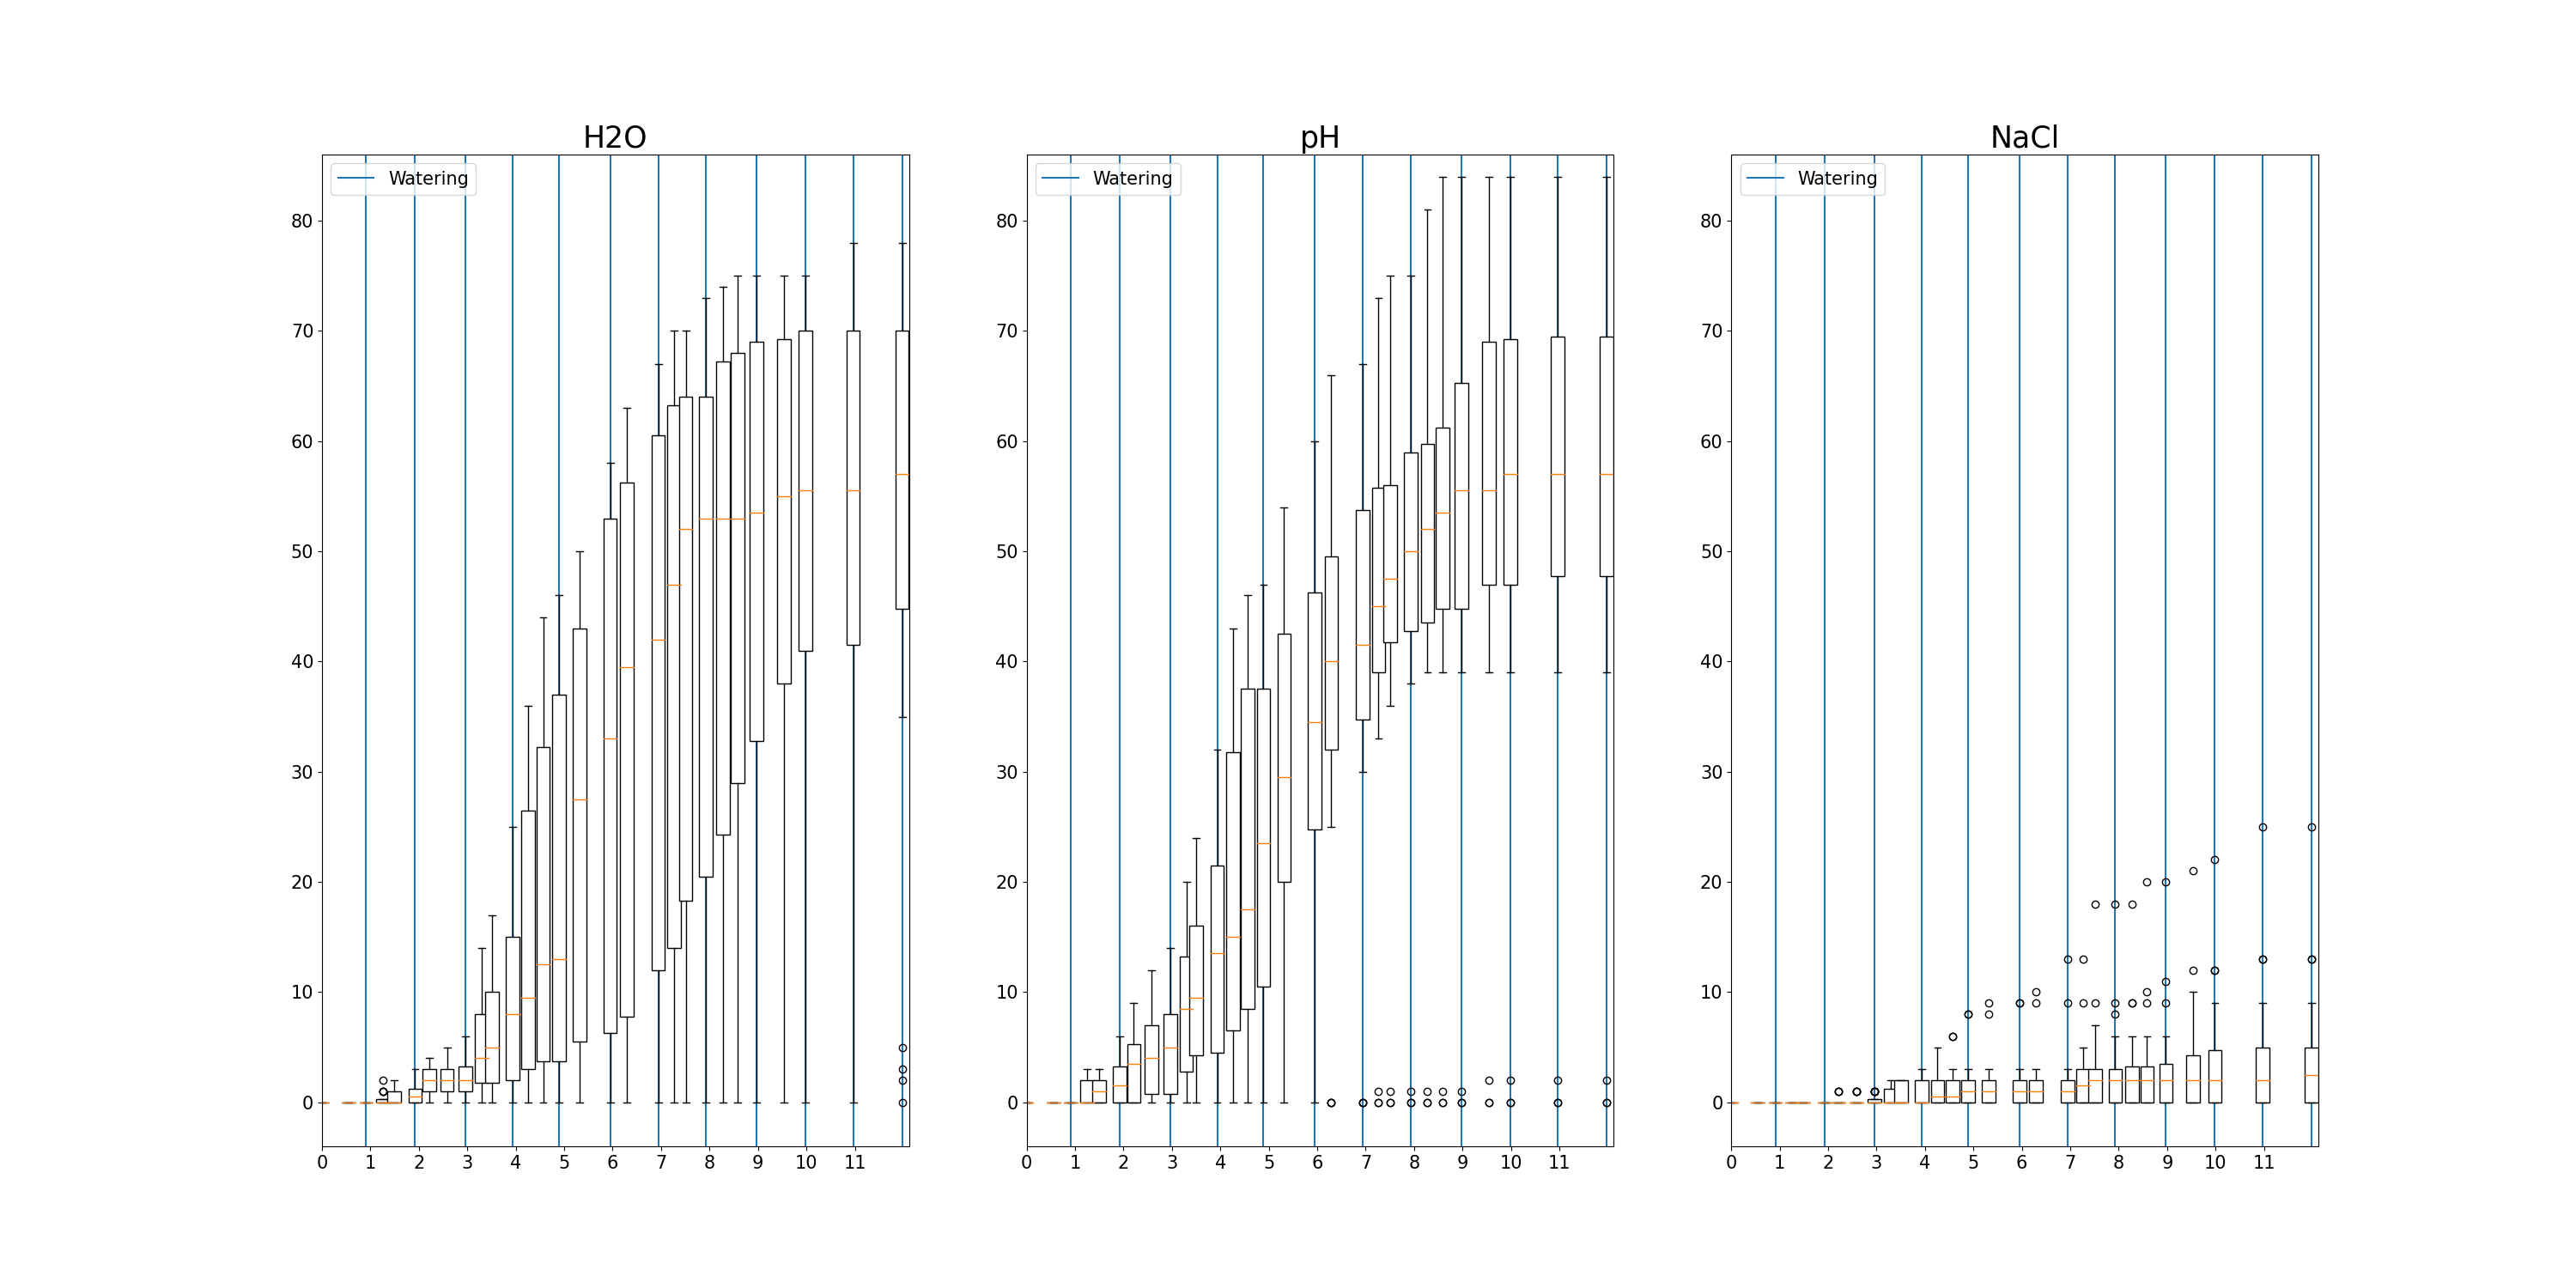
\includegraphics[width=.9\textwidth]{BoxPlot.png}
        \caption{Messwerte als Box-Plot}
        \label{fig:box_plot}
    \end{figure}
    \autoref{fig:box_plot} zeigt alle selbst erhobenen Wuchshöhen, innerhalb der 14 Tage, die das Experiment durchgeführt wurde, als Box-Plot, wobei die teilenden Linien innerhalb der Boxen den Median der jeweiligen Messung darstellen und die Whiskers bis zum ersten Messwert außerhalb der jeweiligen Box reichen.
    \newpage

    \begin{figure}[h]
        \centering
        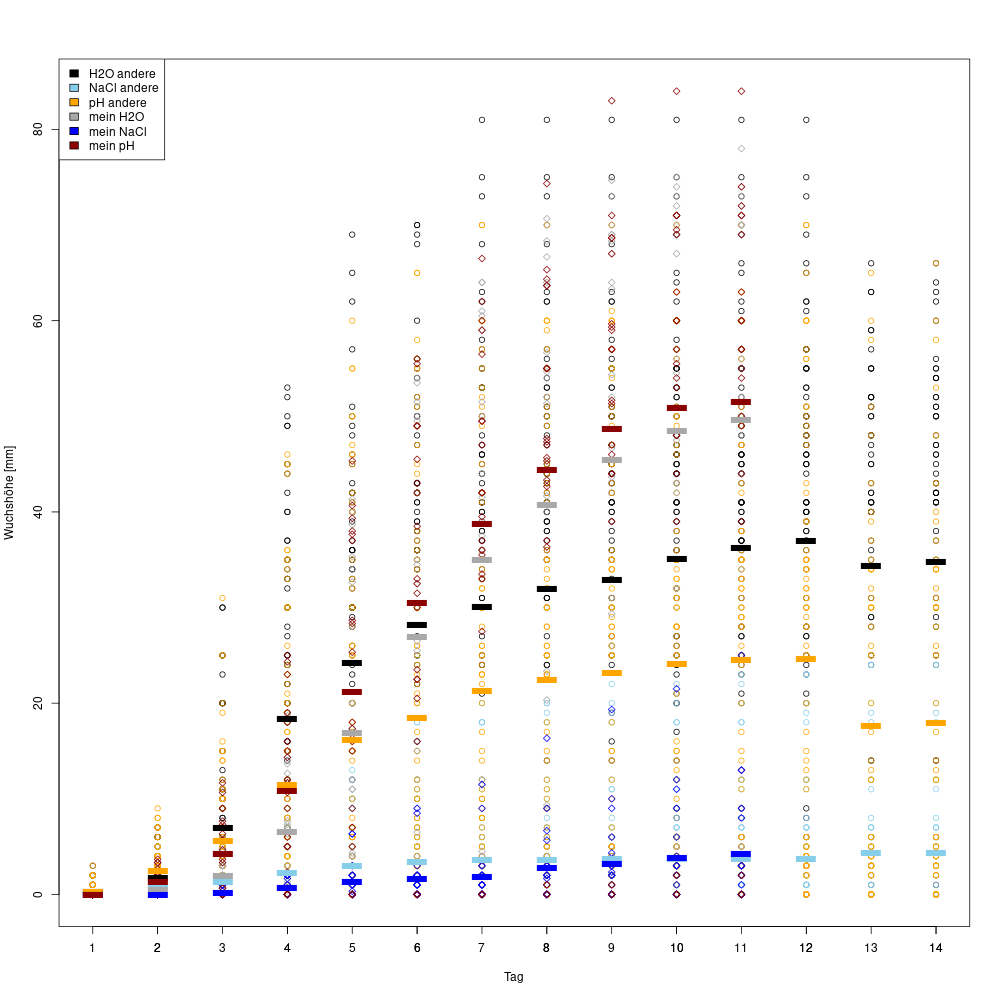
\includegraphics[width=.65\textwidth]{scatterplot_my_vs_others.png}
        \caption{Wertevergleich mit anderen Durchführungen}
        \label{fig:scat_plot_cmp}
    \end{figure}
    In \autoref{fig:scat_plot_cmp} sind alle Messwerte graphisch dargestellt, zusammen mit den Werten aus parallel von anderen Wissenschaftlern durchgeführten Experimenten gleicher Art, als vergleichende Referenz. Hierbei sind die Mittelwerte als dickere Striche abgebildet.

    \begin{figure}[h]
        \centering
        \begin{subfigure}{.32\textwidth}
            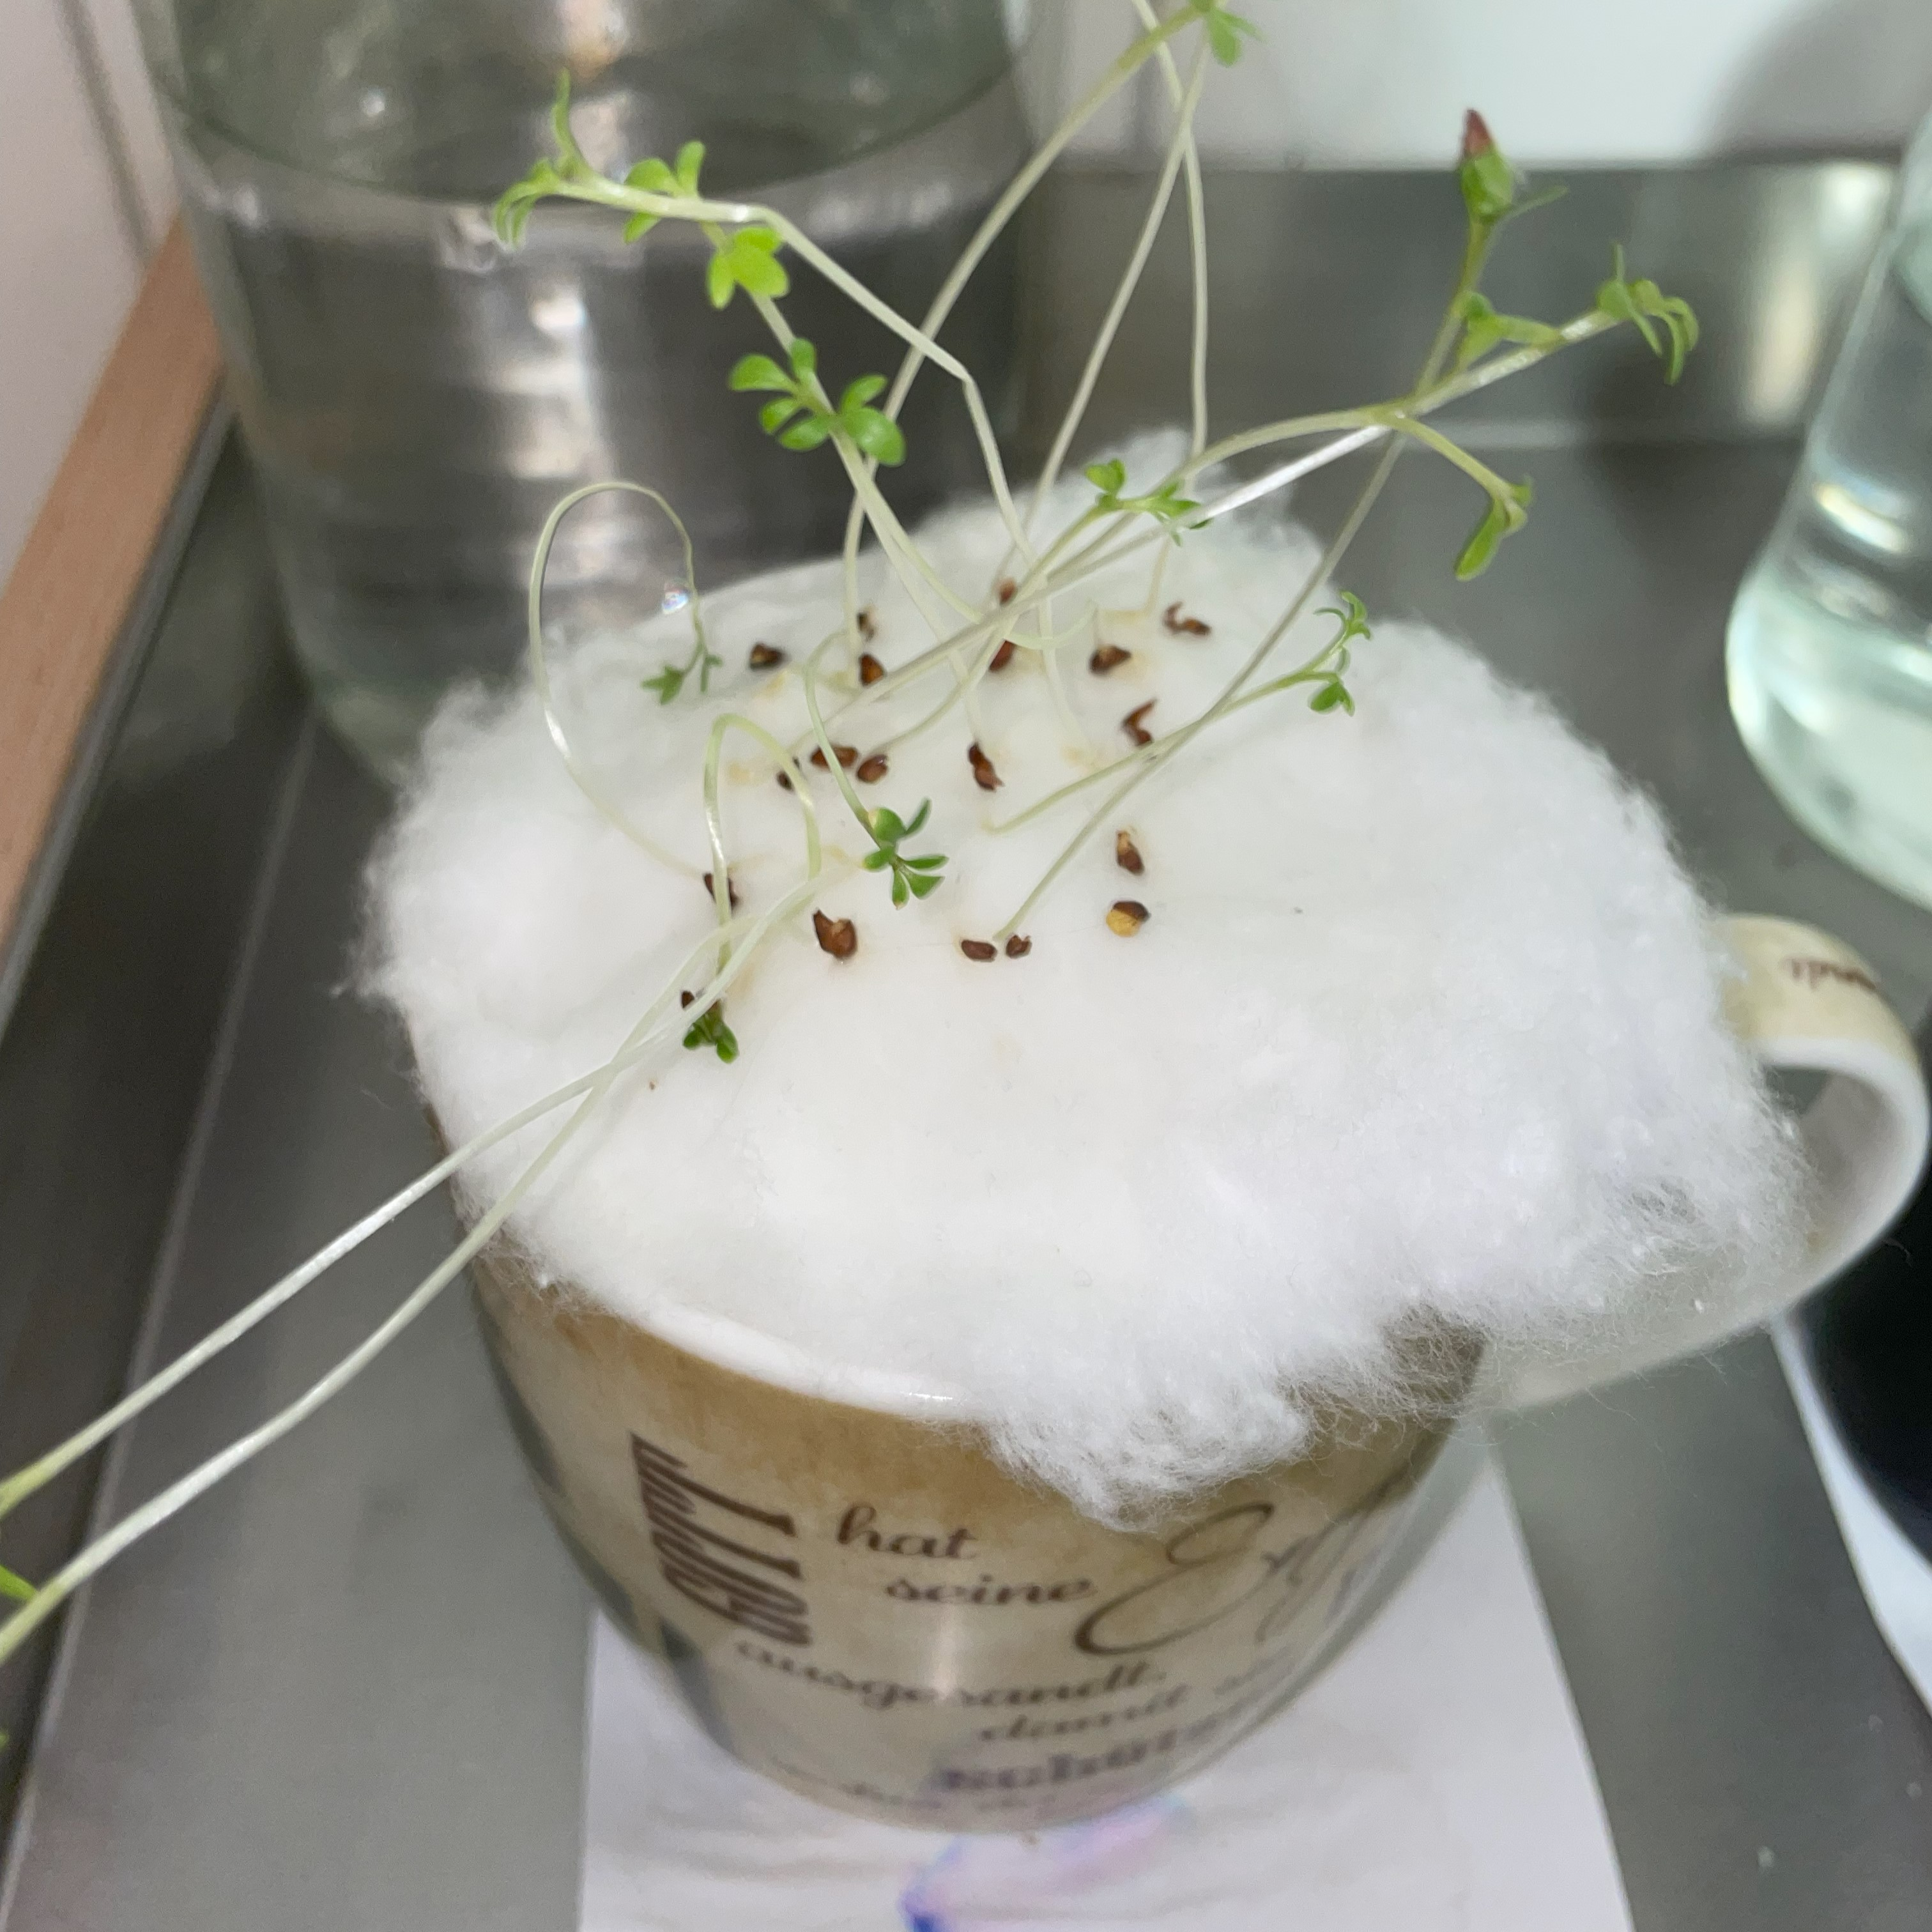
\includegraphics[width=.7\textwidth]{normal_after.png}
            \caption{Normal}
            \label{fig:normal_after}
        \end{subfigure}
        \begin{subfigure}{.32\textwidth}
            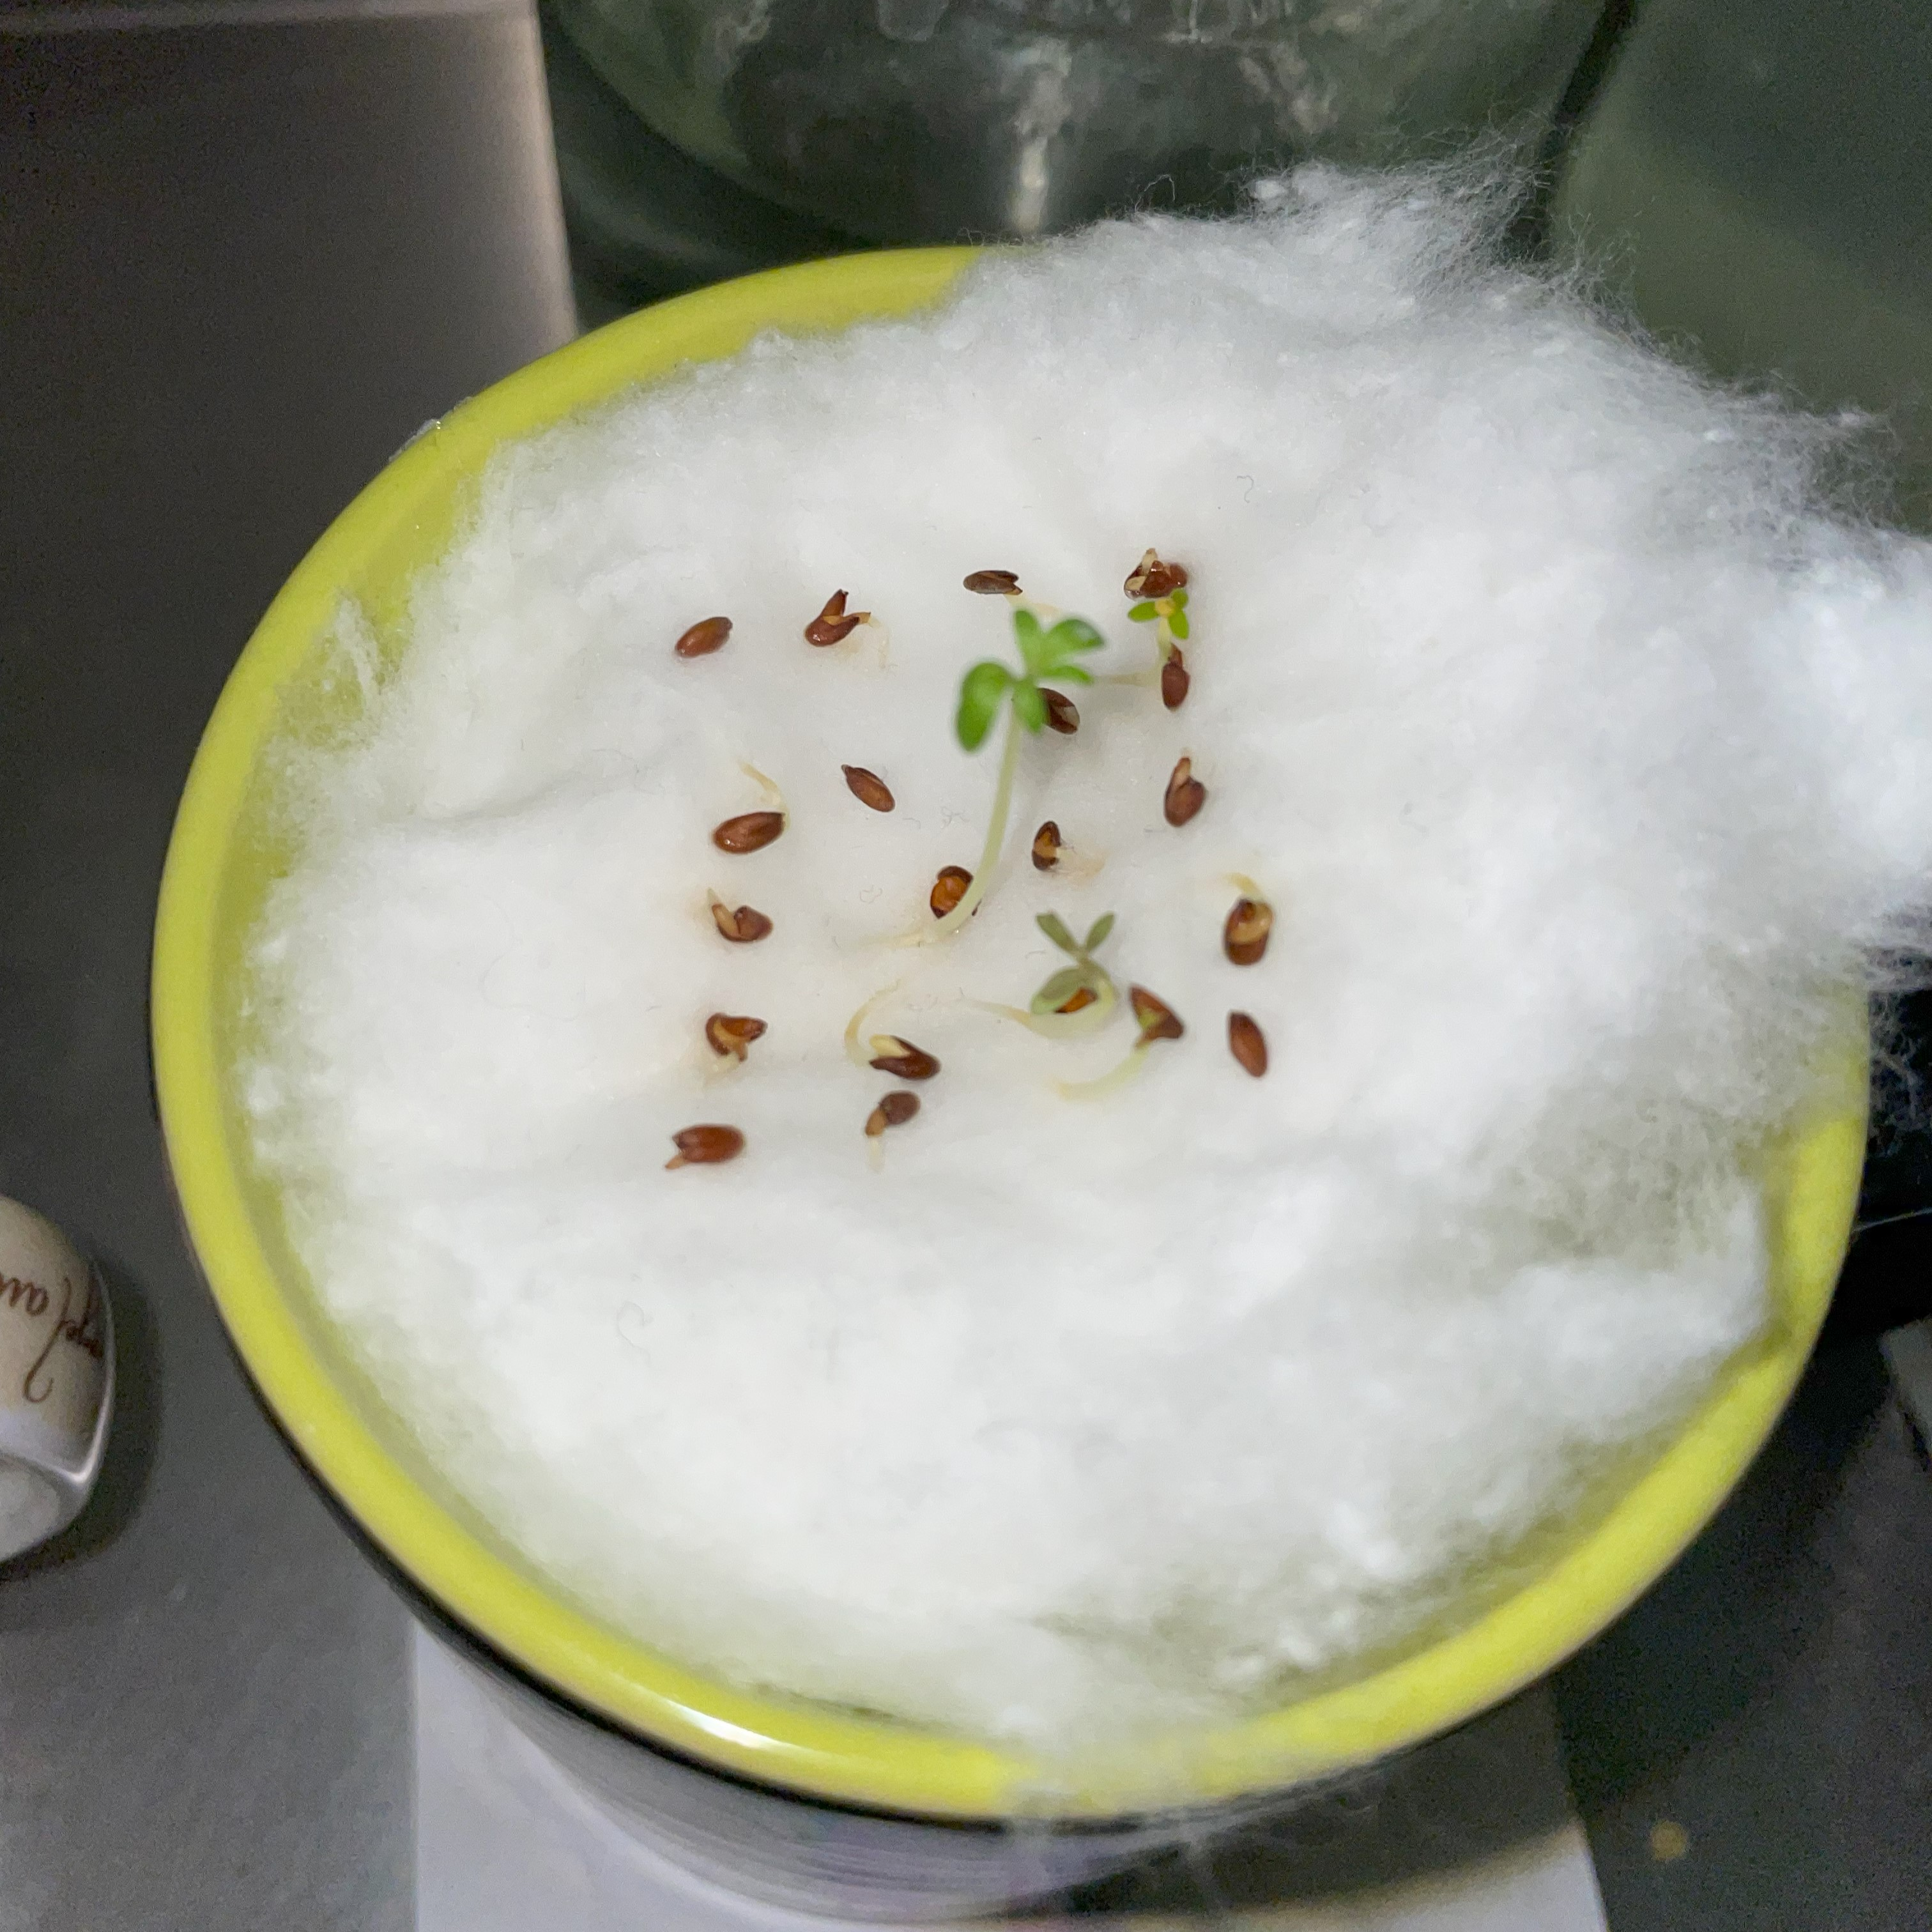
\includegraphics[width=.7\textwidth]{salty_after.png}
            \caption{Salzig}
            \label{fig:salty_after}
        \end{subfigure}
        \begin{subfigure}{.32\textwidth}
            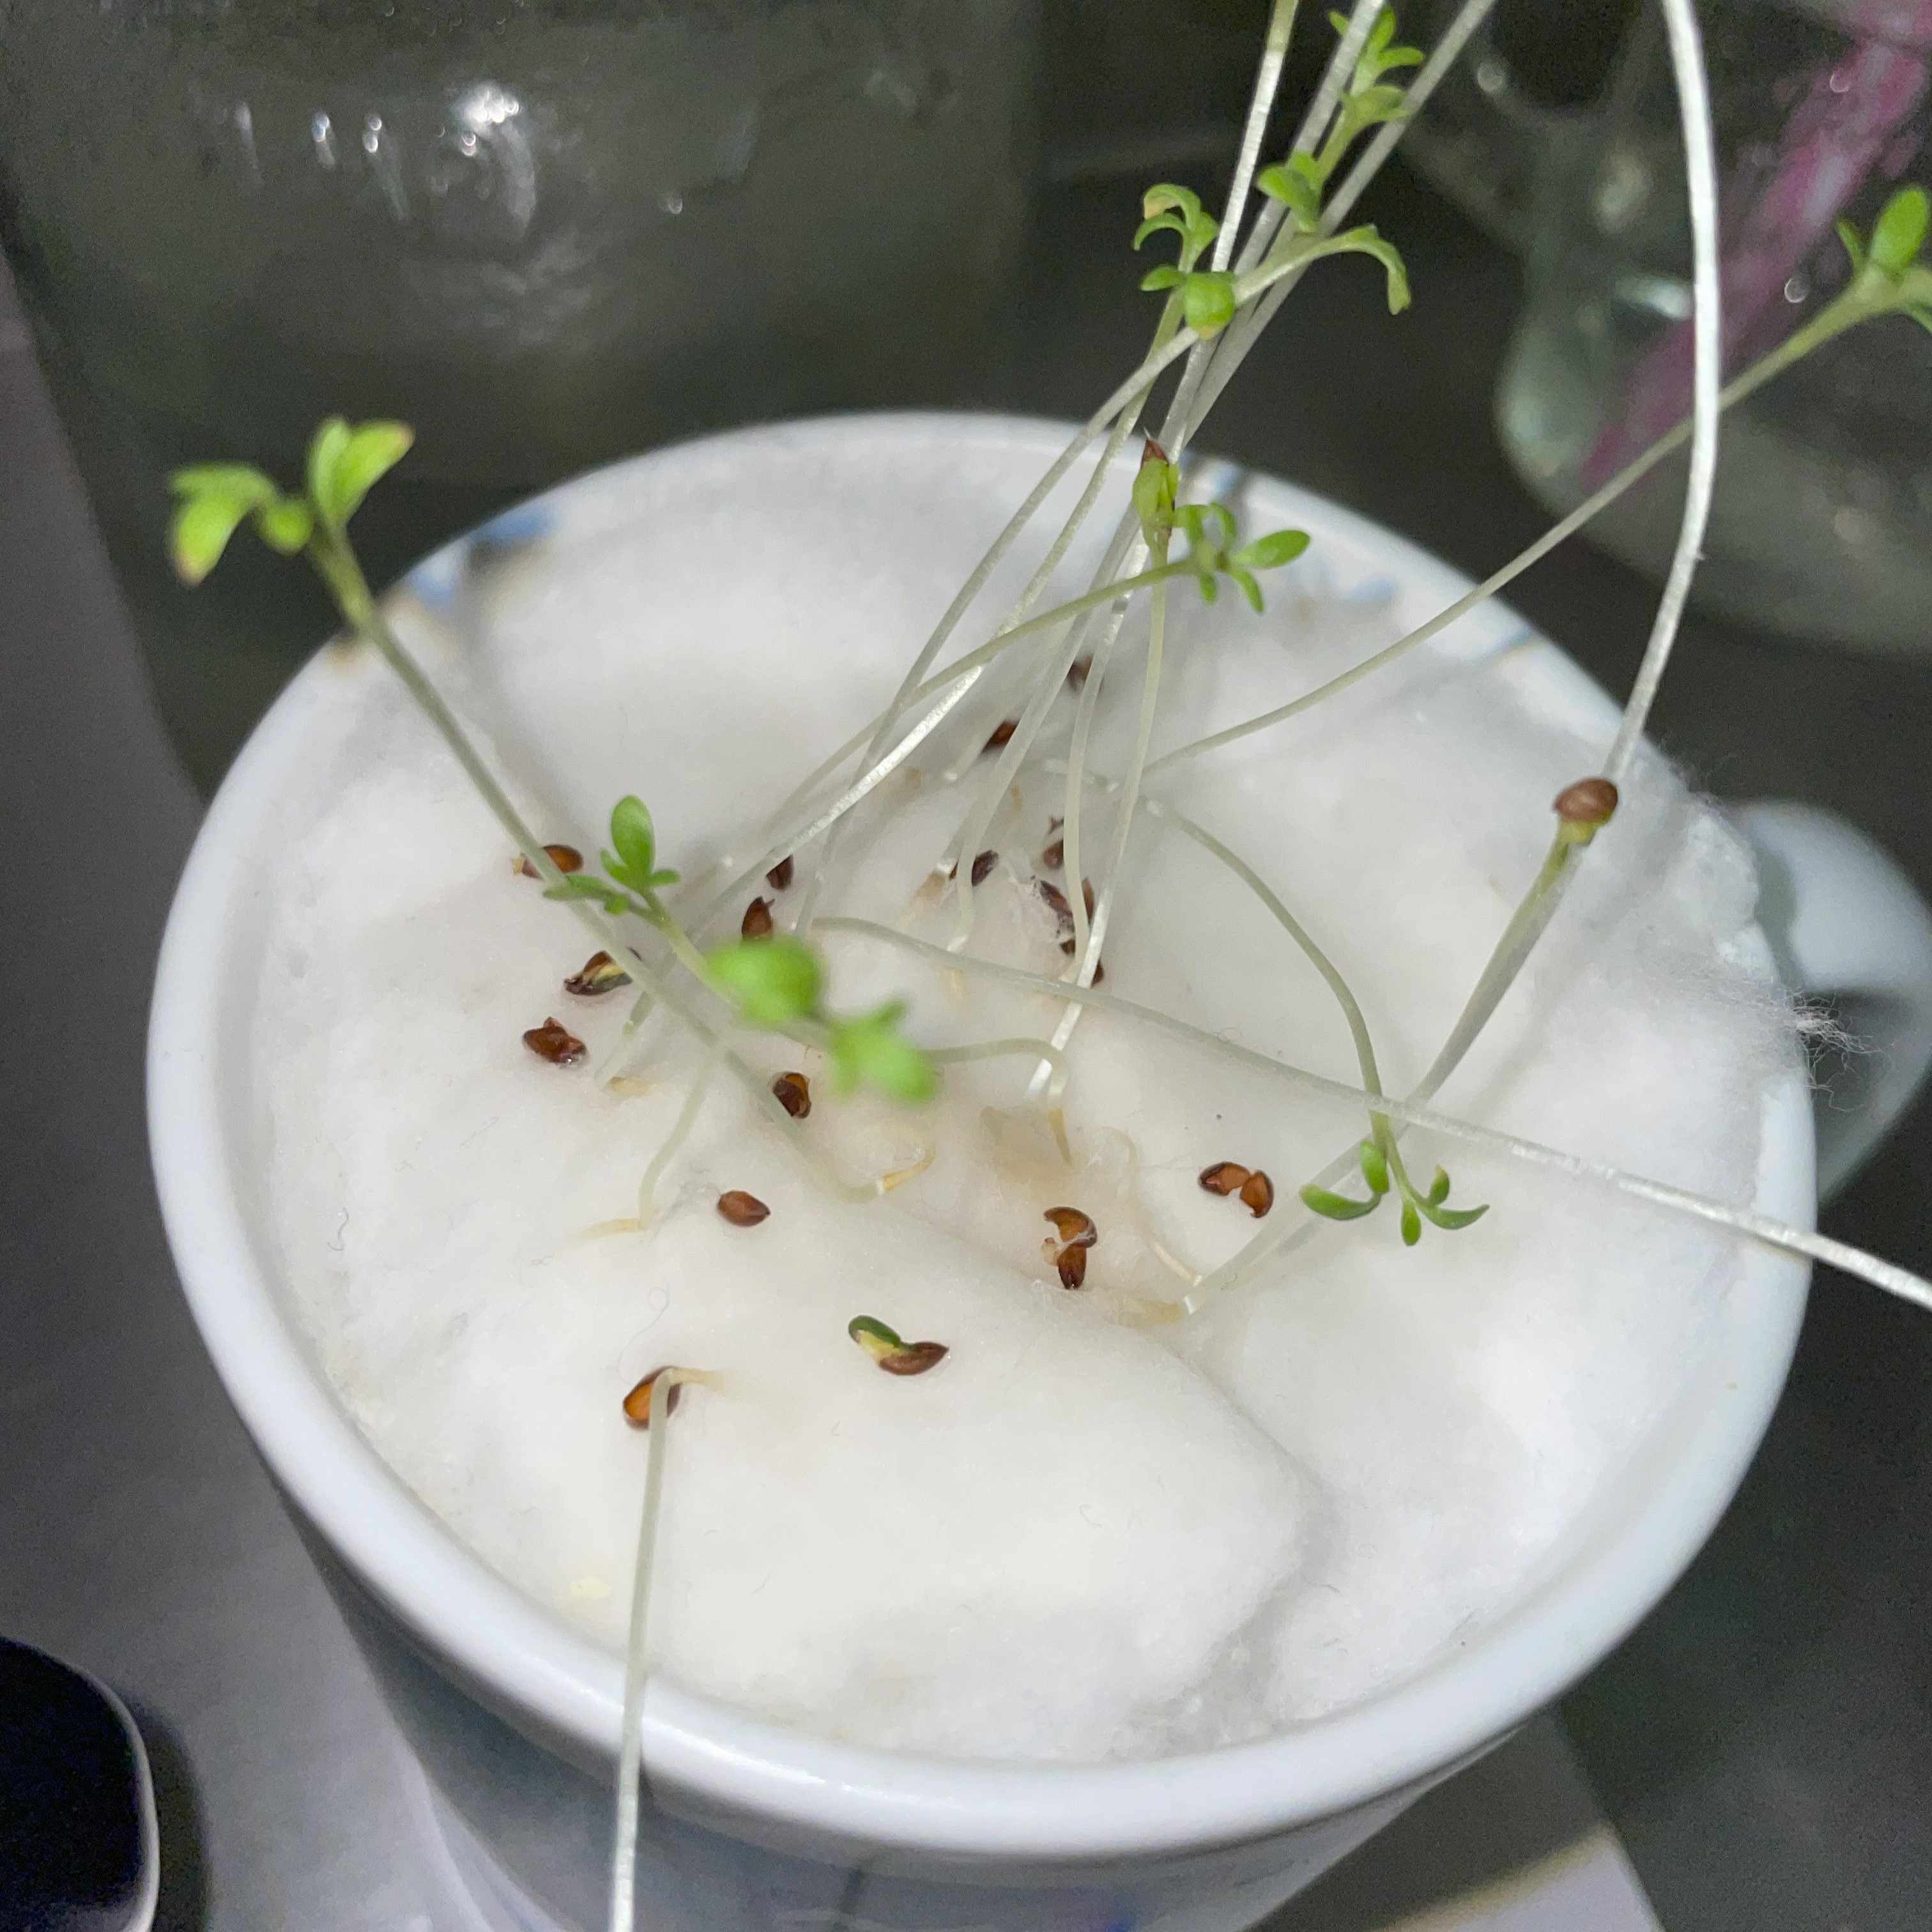
\includegraphics[width=.7\textwidth]{acidic_after.png}
            \caption{Sauer}
            \label{fig:acidic_after}
        \end{subfigure}
        \caption{Pflanzen am letzten Tag}
        \label{fig:exp_after}
    \end{figure}
    \autoref{fig:exp_after} zeigt die Pflanzen der jeweiligen Medien am letzten Tag des Experiments.
% section ergebnisse (end)
